\chapter{Circuit Results Discussion and Summary}
This chapter presents the results of our read-out circuit and the summary of this thesis.
The layout of the circuit is given in \ref{fig:layout}

\begin{figure}[!htbp]
    \centering
    % \includegraphics[width=0.4\textwidth] {images/chapter5/DCMode.png}
    \caption{}
    \label{fig:layout}
\end{figure}

\section{The Fronted Circuit and DC-sweep mode}
\begin{figure}[tbh!p]
    \centering
        \includegraphics[width=0.5\textwidth] {images/chapter5/DCMode.PNG}
    \caption{The fronted circuit}
    \label{fig:frontedCIrcuit}
\end{figure}
As in Fig.\ref{fig:frontedCIrcuit}(a), the fronted circuit includes a biasing current source (Ibias), transimpedance amplifier (TIA) and an operational amplifier (OP).
These three circuit blocks combined with the nanowire device (SiNW) form a feedback structure, which is the DC-sweep mode of our circuit.

\subsection{Ibias}
\begin{figure}[tbh!p]
    \centering
        \includegraphics[width=0.3\textwidth] {images/chapter5/mirror.PNG}
    \caption{The fronted circuit}
    \label{fig:mirror_ch6}
\end{figure}
The Fig.\ref{fig:mirror_ch6} is the schematic of the Ibias.
By changing the resistance of the external Res and measuring the current, we obtained the result shown in Fig.\ref{fig:chip:mirror}.

\subsection{Ibias}

\subsection{TIA}
The Fig.\ref{fig:chip:TIA}(a) and (c) shows that the input current range of TIA is$+5.3\mu A \sim -15\mu A$.
The Fig.\ref{fig:chip:TIA}(b) and (d) are the respective derivative ($\frac{\partial V_{out}}{\partial I_{in}}$), which indicates the TIA has transimpedance of $103k$.
It is notable that not all TIA on the chips have the same transimpedance.
This is because the transimpedance value depends on the resistance of the resistor (Fig.\ref{fig:frontedCIrcuit}).
\emph{We use N-well to implement this resistor, which should have the largest resistance-to-surface ratio among other kinds of resistor.}
But since the doping concentration may vary with the fabrication process, such kind of resistor has a larger resistance variance (\% 30).
We have performed necessary simulation before tap out.
It is assured that the variance does not disturb the important characteristics of whole read-out circuit such as stability and noise ratio.

\begin{figure}[tbh!p]
    \centering
    \begin{minipage}[t]{0.8\textwidth}
        \includegraphics[width=1\textwidth]{images/chapter6/Trimp_I+.png}
        \raggedleft
    \end{minipage}
    \hfill
    \centering
    \begin{minipage}[t]{0.8\textwidth}
        \includegraphics[width=1\textwidth]{images/chapter6/Trimp_I-.png}
        \raggedleft
    \end{minipage}
    \caption{The dc simulation results of TIA. The x-axis represents positive/negative input current (log scale). \textbf{(a)} is the $V_{out}$ responding to the positive input current while \textbf{(c)} is to the negative input current.
                    \textbf{(b)} and \textbf{(d)} are the derivative of $V_{out}$ of input current ($\frac{\partial V_{out}}{\partial {I_{in}}}$) from \textbf{(a)} and \textbf{(c)} respectively.}
    \label{fig:chip:TIA}
\end{figure}




\subsection{OP} \label{sec:ch6:OP}
By applying a sinusoidal signal to the negative input of OP, we found that the gain of OP is about $2k$ (Fig.\ref{fig:chip:OPGain}).
However, the gain of OP was designed to be more than $5k$.

We will discuss this problem in the following section.
\begin{figure}[tbh!p]
    \centering
        \includegraphics[width=0.8\textwidth] {images/chapter6/Problem_OPGain.png}
    \caption{The output voltage of the OP when the negative input is applied with a sinusoidal signal. This input sinusoidal signal has frequency of $1$Hz and amplitude of $1m V$.
            The positive input of OP is biased with a constant voltage generated by the chip.
            The output signal has amplitude around $2 V$, which means that the gain of OP is about $2k$.}
    \label{fig:chip:OPGain}
\end{figure}

\subsection{Measurement with the DC-sweep Mode Circuit and the Low-current Defect Problem}
\begin{figure}[tbh!p]
    \centering
        \includegraphics[width=0.5\textwidth] {images/chapter6/DCMode.png}
    \caption{DC-sweep mode circuit}
    \label{fig:chip:DCmode}
\end{figure}

With the the DC-sweep mode circuit (Fig.\ref{fig:chip:DCmode}), we swept Ibias and measured $V_G$ and $I_D$ to obtain the $I_D$-$V_G$ and $I_{bias}$-$V_G$ curves (Fig.\ref{fig:chip:IdIbiasVG}).
The chip works well when $I_bias$ is larger than $1\mu A$.
The overlap between two curves implies that $I_D$ follows Ibias and $V_G$ consequently alters due to the feedback mechanism.

When current becomes low, the circuit fails to prompt nanowire follows the biasing current.
This phenomenon could be reasonable because the $g_m$ becomes low and the feedback ability of the circuit may be not strong enough to push the gate of nanowire.
However, when design the circuit (chapter 5), we expected this happens for $g_m$ below $200n$.
The Fig.\ref{fig:chip:gmId} indicates the circuit fails when $g_m$ is less than $5\mu$.
We call this problem as the low-current defect.

\begin{figure}[tbh!p]
    \centering
    \includegraphics[width=0.8\textwidth] {images/chapter6/gvt_0101Manual_IdVg.png}
    \caption{The measurement result of the DC-sweep mode circuit. $I_{bias}$ is the biasing current. $I_D$ is the current flowing through the nanowire device.
    One can observe a separation between two curves in low current section ($< 1\mu A$).}
    \label{fig:chip:IdIbiasVG}
\end{figure}

\begin{figure}[tbh!p]
    \centering
        \includegraphics[width=0.7\textwidth] {images/chapter6/gvt_0101Manual_gmId.png}
    \caption{The $g_m$-$I_D$ curve. It is obtained from the $I_D$-$V_G$ curve in Fig.\ref{fig:chip:IdIbiasVG}.
            ``Circuit fails'' means the two curves in Fig.\ref{fig:chip:IdIbiasVG} are separated where ``circuit works'' means they are overlapped.}
    \label{fig:chip:gmId}
\end{figure}

\subsubsection*{Insufficient Gain}
We first suspected that it is caused by the insufficient Op gain (Fig.\ref{fig:chip:DCmode}).
According to the last section (Section.\ref{sec:ch6:OP}), the gain is about $2k$.
The discussion in Section.\ref{sec:feedM} suggests the feedback mechanism depends on the loop gain of the circuit.
The loop gain should be larger than 100 for the DC-sweep mode being functional.
Based on Eq.(\ref{eq:TF_RA}) and Eq.(\ref{eq:TF_LG}), if $A_{OP}$ is $2k$, the loop gain drops below 100 when $g_m$ is less than $500n$.
In other words, even though the gain of OP is 2.5 fold smaller than the gain we designed, the circuit should work well when $g_m$ is larger than $500n$.

One reason may explain is that the gain of OP varies with input.
As depicted in  Fig.\ref{fig:chip:line}, the slope ($\frac{\partial V_{out}}{V_{input}}$) at the midst is larger than the slope at the both end (The slope can represent the gain of OP).
In the measurement of Fig.\ref{fig:chip:OPGain}, the offset of the output signal is around $2V$.
But in Fig.\ref{fig:chip:IdIbiasVG}, when the separation happens, the output voltage of OP ($V_G$) is less than $1.5V$.
Thus, we assert that the gain of OP is less than $2k$.

\begin{figure}[tbh!p]
\centering
    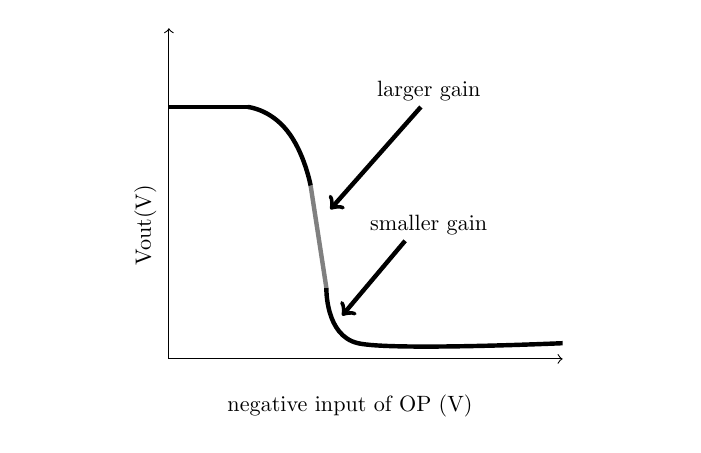
\begin{tikzpicture}
        \draw [black, ultra thick] plot coordinates { (0,4) (1,4) };
        \draw [black, ultra thick] plot [smooth, tension=1] coordinates { (1,4) (1.5,3.7) (1.8,3) };
        \draw [gray, ultra thick] plot [smooth, tension=1] coordinates { (1.8,3) (2,1.7) };
        \draw [black, ultra thick] plot [smooth, tension=0.5] coordinates { (2,1.7) (2.4,1) (5, 1) };

        \draw[->] (0, 0.8) -- (0, 5);
        \draw[->] (0, 0.8) -- (5, 0.8);
        \draw[->, ultra thick] (3.2, 4) -- (2.05,2.7);
        \draw[->, ultra thick] (3, 2.3) -- (2.2,1.35);
        \node[text width=5cm, scale=0.8, align=center] at (3.3, 2.5)
            {smaller gain};
        \node[text width=5cm, scale=0.8, align=center] at (3.3, 4.2)
            {larger gain};
        \node[text width=10cm, scale=0.8, align=center] at (2.3, 0.2)
            {negative input of OP (V)};
        \node[text width=5cm, scale=0.8, align=center, rotate=90] at (-0.3, 2.5)
            {Vout(V)};
    \end{tikzpicture}
    \caption{}
    \label{fig:chip:line}
\end{figure}


\subsubsection*{Input Offset Voltage}
Another reason may be responsible for the low-current defect is the offset voltage at the input of the OP.

We examined the output voltage of TIA ($V_{TIA}$) of the Fig.\ref{fig:chip:IdIbiasVG} DC-sweep experiment.
It is shown in Fig.\ref{fig:chip:VTIA}.
Ideally, when feedback mechanism works well, $V_{TIA}$ should be equal to $V_{Ref}$(Fig.\ref{fig:chip:DCmode}).
However, the value of $V_{Ref}$ is $0.802 V$, which is smaller than $V_{TIA}$.
(This $V_{Ref}$ is connected to a constant voltage point inside the chip.
We know its value indirectly by measuring the drain voltage of nanowire since the drain of nanowire is kept to be same as $V_{Ref}$ by TIA.)
When the circuit works well, $V_{TIA}$ and $V_{Ref}$ is still different by $15m V$.
This voltage difference can result in an $150n A$ offset current flowing through TIA and into the nanowire device.
This offset current becomes remarkable when the $I_{bias}$ is less than $1\mu A$.

We suggest the reason that $V_{TIA}$ is large than $V_{Ref}$ is due to the offset voltage appearing at the input of the OP.
This speculation is reasonable through with respect to the layout, which will be discussed in the next section.

\begin{figure}[tbh!p]
    \centering
        \includegraphics[width=0.7\textwidth] {images/chapter6/gvt_0101Manual_VopiProblem.png}
    \caption{The $V_{TIA}$. The x-axis is the corresponding gate voltage.
                With the information from Fig.\ref{fig:chip:IdIbiasVG}, we found that the $V_{TIA}$ is not equal to $V_{Ref}$ no matter feedback mechanism works well or not.}
    \label{fig:chip:VTIA}
\end{figure}

Overall, the insufficient gain and the input offset may be the main reasons of the low-current defect.
Both of them relate to the OP block.
We then discuss these two reasons from the perspective of layout.

\subsection{The Design and Layout Problems of OP}
In the last section, me mentioned that the gain of OP is lower than we expected and there may exist an input offset voltage.
In this section, we will deduce that several layout flaws may be responsible for these two problems.

\begin{figure}[tbh!p]
    \centering
    \includegraphics[width=1\textwidth] {images/chapter6/OP_schematic.png}
    \caption{The left section is the schematics of the OP and the local biasing circuit. The right section is the global biasing circuit for generating two global biasing voltages: $V_{bi}$, $V_{Ref}$.
                The Iin is an external current source.}
    \label{fig:chip:OPScem}
\end{figure}

\begin{figure}[tbh!p]
    \centering
    \includegraphics[width=0.7\textwidth] {images/chapter6/TrOP_layout.PNG}
    \caption{The layout of the OP including the local biasing circuit (The transistor Mc1$\sim$3 in Fig.\ref{fig:chip:OPScem}) }
    \label{fig:chip:OPLayout}
\end{figure}

\subsubsection{The Possible Reasons for Insufficient Gain}
The schematic presented in Fig.\ref{fig:chip:OPScem} contains two sections.
The left section is the body of the OP, while the right one is a global biasing circuit.
The global biasing circuit generated $V_{bi}$ and $V_{Ref}$, which bias two pmos (M3, M4) and two nmos (M5, M6) respectively.

One layout flaw is that the M3 $\sim$ M6 are all single transistor.
They are placed alone on the chip (Fig.\ref{fig:chip:OPLayout}) without any protection, which cause their size and doping concentration to be vulnerable to the process variation.
Another layout flaw is that the global biasing circuit is not placed next to the OP circuit.
The extent of the process variation from which the OP circuit and global biasing circuit suffer may be different.

Take an example, when process variation happens in global biasing circuit, $V_{bi}$ and $V_{Ref}$ change respectively.
Ideally, the effect of these two changes on the gain of OP are countervailing.
But this may not be true if M4 and M6 suffer distinct process variation and response differently to the gate voltage difference.
Moreover, the high output impedance of OP amplifies this difference.
Hence, the gain of the OP we design is more sensitive to the process variation.

\subsubsection{The Possible Reasons for Input Offset}
The input offset can be related to the size mismatch between M7 and M8 (Fig.\ref{fig:chip:OPLayout}).
There is no dummy gate or matching technique applied to the transistors.
Therefore, the size mismatch may prone to happen on M7 and M8.
In our case, the offset voltage is negative ($V_{\text{negative input}} > V_{\text{positive input}}$).
This means that the size of M8 may be relatively smaller than M7 (We designed them to be same).

\subsubsection{Improvement Methodology}
Although all problems mentioned above relate to the layout, we do not think that simply revising the layout is a reliable solution.
The OP is a high an open-loop circuit with high output impedance.
Its characteristics (such as gain) are hard to be control accurately considering the process variations.
A better solution will be replace the OP.
This OP served as a high-gain and low bandwidth block.
In the future, we can substitute a close-loop amplifier and low pass filter for it.


\section{The Second Stage Circuit and Transient Measurement Mode}
\begin{figure}[tb!hp]
    \begin{minipage}[t]{0.5\textwidth}
        \centering
        \includegraphics[width=1\textwidth]{images/chapter6/NWROC_block.png}
        \raggedleft
        (a)
    \end{minipage}
    \hfill
    \begin{minipage}[t]{0.5\textwidth}
        \centering
        \includegraphics[width=1\textwidth]{images/chapter6/Second.png}
        \raggedleft
        (b)
    \end{minipage}
    \caption{\textbf{(a)} The block diagram of the Transient Measurement mode circuit. \textbf{(b)} The schematic of the second stage circuit.}
    \label{fig:chip:ACschem}
\end{figure}

As in Fig.\ref{fig:chip:ACschem}, the Transient Measurement mode includes the Ibias and TIA from the fronted circuit and the second stage circuit.
An analog subtractor and a resistor-based amplifier are included in the second-stage circuit.
The input signal can be sent from the gate or the source of nanowire (SiNW) as mentioned in chapter 5.


\subsubsection{Summary of DC-sweep mode}

{\color{red}The low current defect problem is not ignorable.
The }
% appropriate operation region
% g_m is not low

\subsection{The Second Stage Circuit}
We present the important circuit properties in this section.
To be notable that we did not measure the performance of the subtractor and amplifier independently because there is no any external pad connected to the output of the subtractor.
Besides, the output of TIA is always connected with the second stage input.
Due to the low output impedance of the TIA, it is hard to give the input signal of the second stage circuit directly.
Fig.\ref{fig:chip:MeasMethod} is the alternative approach.
The resistor Rs and the TIA compose a voltage amplifier.
By injecting input signal through the Rs, we can therefore obtain the correct input and output signal of the second stage circuit.

\begin{figure}[tbh!p]
    \centering
    \includegraphics[width=0.7\textwidth] {images/chapter6/CVMVsMeas.png}
    \caption{}
    \label{fig:chip:MeasMethod}
\end{figure}



\subsubsection{Noise Oscillation Problem in Amplifier with Amplification Rate of 1  }
The amplifier in the second stage circuit has three amplification rate ($A_{amp}$): 1, 10 and 100.
The amplifier works well as the $A_{amp}$ is 10 and 100.
However, when $A_{amp}$ is 1, the output signal is flooded with noise.
In Fig.\ref{fig:chip:ss_noise}, a 1Hz triangle signal is sent to the Rs.
By the voltage amplifier composed of Rs and TIA, the signal is then sent into the second stage circuit.
Ideally, the second stage output should be a triangle signal as well.
But in fact the signal is flooded with noise.
\begin{figure}[tbh!p]
    \centering
    \includegraphics[width=1\textwidth] {images/chapter6/Subtractor_noise.png}
    \caption{}
    \label{fig:chip:ss_noise}
\end{figure}

We suggest that the oscillation of noise signal should be the main cause of the problem.
The simulation we performed in chapter 5 did not consider the parasitic capacitance brought by the pad (with ESD circuit) at the output and switches.
The new simulation proves our suggestion.
The second dominant pole locates at the output.
The parasitic capacitors push it to the left and decrease the phase margin.



\begin{figure}[tbh!p]
    \centering
    \includegraphics[width=1\textwidth] {../images/chapter6/SeconStage_feed.png}
    \caption{}
    \label{fig:chip:ss_feed}
\end{figure}

The reason that the noise oscillation problem only happens when $A_{amp}$ is 1 is because of the feedback mechanism.
The two switches of amplifier are turned off (Fig.\ref{fig:chip:ACschem}(b)).
The structure is similar to an unit-gain buffer.
In Fig.\ref{fig:chip:ss_feed}, (a) is the feedback network of this structure while (c) is of the amplifier with gain of 10 and 100.
To compute the loop gain, the structure is broken at the negative input and a test signal is injected ($Vt$) as illustrated in Fig.\ref{fig:chip:ss_feed} (b), (d).
The loop gain ($\frac{V_f}{Vt}$) of the two structure is derived as:
\begin{align}
    & \text{when $A_{amp} = 1$:} && \frac{V_f}{Vt} = A_{op} \\
    & \text{when $A_{amp} = 10$ or $100$:} && \frac{V_f}{Vt} = A_{op} \times \frac{R_i}{R_i + R_o}
\end{align}
$A_{op}$ is the gain of the OP in the amplifier where the loading effect has been taken into consideration.
Since the $R_O$ is at least larger than $R_i$ by 10-fold, the two loop gain is different by 10-fold as well.
The smaller loop gain increases the phase margin of amplifier by about 45 degree and diminish the oscillation.



{\color{red}Although the noise oscillation problem exist, we can still recognize the trend of the output signal by applying the signal average technique.
The side effect of this technique is that it induce an offset ($\approx 0.15 V$) to the output signal.
This will appears in the following section where the input dynamic range is measured.}

\subsubsection{Dynamic Input Range}
Fig.\ref{fig:chip:xin} is the input-output response of the second stage circuit ($A_{amp} = 1$).
We find the dynamic input range of the circuit with it.
As illustrated in the figure, the linear region locates at $Vin = 0.62V \sim 1.32V$.
According to chapter 5, this range is determined by the subtractor block.
\begin{figure}[tbh!p]
    \centering
    \includegraphics[width=0.6\linewidth] {images/chapter6/SubtractorXin.png}
    \caption{The input-output response of the second stage circuit.}
    \label{fig:chip:xin}
\end{figure}

Another input of the circuit is the Vz (Fig.\ref{fig:chip:ACschem}).
This voltage is for shifting the offset voltage.
Its dynamic input range is measured and presented in Fig.\ref{fig:chip:zin}, which ranges from $0.43V$ to $1.28V$.
To be notable that ideally the input Vz should be equal to the output.
But in fact an offset voltage occurrs in Fig.\ref{fig:chip:ACschem} due to the noise oscillation problem mentioned in the last section.
This offset does not exist when the $A_{amp}$ is 10 and 100.
\begin{figure}[tbh!p]
    \centering
    \includegraphics[width=0.6\linewidth] {images/chapter6/SubtractorZoffset.png}
    \caption{The input-output response of the second stage circuit. The input is Vz, which is decide the output offset of the circuit.}
    \label{fig:chip:zin}
\end{figure}

\subsubsection{The Circuit Gain}
The second stage circuit has three gain: 1, 10 and 100.
We send a triangle wave to the end of Rs (Fig.\ref{fig:chip:MeasMethod}) and measure the input and output of the second stage circuit.
Fig.\ref{fig:chip:amp}) (a), (b) and (c) are the results of the second stage circuit with amplification rate of 1, 10 and 100 respectively.
The exact gain values are summarized in the end of the section (Table.\ref{tb:chip:ampGain}).


\begin{figure}[tbh!p]
    \centering
    \begin{minipage}[t]{1\linewidth}
        \includegraphics[width=0.8\linewidth] {images/chapter6/SubtractorXin_scope.png}
        \raggedleft (a)
    \end{minipage}
    \centering
    \begin{minipage}[t]{1\linewidth}
        \includegraphics[width=0.8\linewidth] {images/chapter6/SecondStageAmp10x.png}
        \raggedleft (b)
    \end{minipage}
    \begin{minipage}[t]{1\linewidth}
        \centering
        \includegraphics[width=0.8\linewidth] {images/chapter6/SecondStageAmp100x.png}
        \raggedleft (c)
    \end{minipage}
    \caption{}
    \label{fig:chip:amp}
\end{figure}

\begin{table}
    {\fontfamily{}\fontsize{10}{14}\selectfont
    \centering
    \begin{tabular}{l|c|c|c}
        Designed Amplification Rate & 100 & 10 & 1 \\
        \hline
        Measured Amplification Rate & 93.3 & 9.2 & 1 \\
        \hline
        Error Rate & 7.7 \% & 8 \% & 0 \\
    \end{tabular}
    \caption{}
    \label{tb:chip:ampGain}
    }
\end{table}

\subsection{Transient Measurement Mode}
The TIA from the fronted circuit and the second stage circuit compose the circuit of Transient Measurement Mode.
This section presents the important properties of the circuit (gain, noise and bandwidth).


\subsubsection{Bandwidth and Gain}

\begin{figure}[tbh!p]
    \centering
    \begin{minipage}[t]{1\linewidth}
        \centering
        \includegraphics[width=0.8\linewidth] {images/chapter6/Bw_10x.png}
        \raggedleft (a)
    \end{minipage}
    \centering
    \begin{minipage}[t]{1\linewidth}
        \centering
        \includegraphics[width=0.8\linewidth] {images/chapter6/Bw_100x.png}
        \raggedleft (b)
    \end{minipage}
    \caption{}
    \label{fig:chip:bw}
\end{figure}
The gain is the input current to output voltage ratio.
Because the noise oscillation problem may disturb the bandwidth measurement, we did not measure the circuit with $A_{amp}$ of 1.
The circuit with $A_{amp}$ of 10 has gain of $891k$ and bandwidth of $30k$Hz.
The circuit with $A_{amp}$ of 100 has gain of $8.9M$ and bandwidth of $7.5k$Hz.

\subsubsection{Input Referred Noise}
The spectrum analyzer are used to measure the noise.
We measure the power spectral density (PSD) of noise at the output of the circuit and refer it to the input to show the equivalent input current noise.
As illustrate in Fig.\ref{fig:chip:noise}, the primary type of noise are the low frequency noise, especially the $60$Hz environmental noise.
The environmental noise may be lowered by adopting better method of experiment or equipment.
Overall, the amount of noise is tolerable.
The spec. from chapter 3 allows for a maximal input current noise of $2n A$.

\begin{figure}[tbh!p]
    \centering
    \includegraphics[width=0.8\linewidth] {images/chapter6/Noise.png}
    \caption{}
    \label{fig:chip:noise}
\end{figure}


\subsubsection{Modulating biomolecule signals from the source terminal}
The second usage of the Transient Measurement mode circuit is to apply a sinusoidal signal at the source of nanowire.
In Fig.\ref{fig:chip:sin}, we injected a $500$Hz sinusoidal signal with amplitude of $0.5V$ into the source of nanowire and measured the output.
The nanowire was put under two solutions with different pH values in (a) and (b).
After dividing the amplitude of the output signal by the transimpedance gain of the circuit (891k), we learned that the $g_m$ of nanowire under these two pH solutions are $1\mu$ and $1.8\mu$.

This method aims to modulate the biomolecule signal into higher frequency to avoid the flicker noise and other kinds of low frequency noise.
However, from the result blow, we observe that the output contains large amount of high frequency noise.
We believe the noise comes through the gate of nanowire which is covered by the testing solution.
In the future, a bandpass filter with adjustable center frequency should be added into the circuit.

\begin{figure}[tbh!p]
    \centering
    \begin{minipage}[t]{1\linewidth}
        \includegraphics[width=0.8\linewidth] {../images/chapter6/Sin_1u.png}
        \raggedleft (a)
    \end{minipage}
    \centering
    \begin{minipage}[t]{1\linewidth}
        \includegraphics[width=0.8\linewidth] {../images/chapter6/Sin_1p8u.png}
        \raggedleft (b)
    \end{minipage}
    \caption{}
    \label{fig:chip:bw}
\end{figure}


\subsubsection{Summary of Transient Measurement mode}
The table that compares the chip properties and the specification for transient measurement mode is given below (Table.\ref{tb:chip:cvmR}).
Although there is the noise oscillation problem, the overall performance of the circuit is as expected.


\begin{table}[tbh!]
    {\fontfamily{}\fontsize{10}{14}\selectfont
    \centering
    \begin{tabular}{l|c|c}
        & Design Spec. & Chip Properties  \\
        \hline
        \hline
        $\Delta I_D$ & $\pm 2.8\mu A$ & $5.3\mu A$-$-15\mu A$\\
        \hline
        Input Referred Current Noise &$< 2n A$ & $< 0.5n A$\\
        \hline
        Transimpedance Gain (max) & $5 M(\frac{V}{A})$& $8.9 M (\frac{V}{A})$\\
        \hline
        Bandwidth &$> 1k$ (Hz) & $7.5k Hz$\\
    \end{tabular}
        \caption{The comparison between the chip properties and the specification for transient measurement mode from chapter 3.}
        \label{tb:chip:cvmR}
    }
\end{table}


\section{Dealing with the Device Variability Problem}
This section presents the measurement with the proposed variability-resisting method.

Two nanowire devices (nw1-2, nw2-1) lying on the same substrate are under test.
The $I_D$-$V_G$ curves of two devices are obtained and substantiate that they have device variability problem (Fig.\ref{fig:chip:DeviceVar}(a)).
These curves are then transformed into $gm$-$Id$ curves (Fig.\ref{fig:chip:DeviceVar}(b)).
Based on the conclusion of appropriate operation region (Section.\ref{section:biasVg}), the $gm$ of $2\mu$ is selected.
The certain $I_D$ under which devices are biased are therefore determined.
As illustrated in Fig.\ref{fig:chip:DeviceVar}(b), nw1-2 is biased under $340n A$ and nw2-1 is biased under $900n A$.
The devices are connected with the circuit in transient measurement mode, where the bias current and gate voltage are set.
Finally, the output response of two devices are presented in Fig.\ref{fig:chip:DeviceVar}(c) and (d).
Two solutions with different pH values is used in substitution for the DNA solution.
The pH value of solution A is lower than solution B.
The lower pH value means the solution is more positive.
Thus, solution B increase $I_D$ and increases output voltage.

Two devices have similar output response, which suggest our method is functional.
But still the responses are not exactly same.
We can blame the inaccurate biasing current because the DC-sweep mode circuit fails in low current and the $V_G$ is manually adjusted to make the $I_D$ follows the biasing current.
However, we suggest it relates to the equivalent voltage change induced by the concentration (pH value) difference ($\Delta V$).
Although we keep the devices under a same $gm$, the output signals can diverge if they receive incomparable input.



\begin{figure}[bth!]
    \centering
    \begin{minipage}[t]{0.4\linewidth}
        \includegraphics[width=1\textwidth] {../images/chapter6/DeviceVar_IdVg.png}
        \raggedleft (a)
    \end{minipage}
    \centering
    \begin{minipage}[t]{0.55\linewidth}
        \includegraphics[width=1\textwidth] {../images/chapter6/DeviceVar_gmId.png}
        \raggedleft (b)
    \end{minipage}
    \begin{minipage}[b]{1\linewidth}
        \includegraphics[width=1\textwidth] {../images/chapter6/DeviceVar_scope.png}
        \makebox[0.4\linewidth][r]{ (c)}
        \makebox[0.57\linewidth][r]{ (d)}
    \end{minipage}
    \caption{}
    \label{fig:chip:DeviceVar}
\end{figure}


Because of the low current defect problem, the first step: $I_D$-$V_G$ sweep is not performed by DC-sweep mode but by the source meter.
















%
